\documentclass{article}

% if you need to pass options to natbib, use, e.g.:
%     \PassOptionsToPackage{numbers, compress}{natbib}
% before loading neurips_2018

% ready for submission
% \usepackage{neurips_2018}

% to compile a preprint version, e.g., for submission to arXiv, add add the
% [preprint] option:
%     \usepackage[preprint]{neurips_2018}

% to compile a camera-ready version, add the [final] option, e.g.:
\usepackage[final]{nips_2018}

% to avoid loading the natbib package, add option nonatbib:
%     \usepackage[nonatbib]{neurips_2018}

\usepackage[utf8]{inputenc} % allow utf-8 input
\usepackage[T1]{fontenc}    % use 8-bit T1 fonts
\usepackage{hyperref}       % hyperlinks
\usepackage{url}            % simple URL typesetting
\usepackage{booktabs}       % professional-quality tables
\usepackage{amsfonts}       % blackboard math symbols
\usepackage{nicefrac}       % compact symbols for 1/2, etc.
\usepackage{microtype}      % microtypography
\usepackage{amsmath}
\usepackage{algorithm,algorithmic}
\usepackage{graphicx}
\usepackage{bbm}


\newcommand{\fracpartial}[2]{\frac{\partial #1}{\partial  #2}}
\newcommand{\Dir}[0]{\textrm{Dirichlet}}
\newcommand{\Ray}[0]{\textrm{Rayleigh}}
\newcommand{\gam}[0]{\textrm{Gamma}}
\newcommand{\dgamma}[0]{\textrm{Gamma}}
\newcommand{\dpoisson}[0]{\textrm{Poisson}}
\newcommand{\dbeta}[0]{\textrm{Beta}}
\newcommand{\dbern}[0]{\textrm{Bernoulli}}
\newcommand{\dunif}[0]{\mathrm{Uniform}}
\newcommand{\dgig}[0]{\textrm{GIG}}
\newcommand{\dnormal}[0]{\mathrm{Normal}}
\newcommand{\dt}[0]{\mathrm{t}}
\newcommand{\igamma}[0]{\textrm{Gamma}^{-1}}
\newcommand{\rayl}[0]{\textrm{Rayleigh}}
\newcommand{\Exp}[0]{\textrm{Exponential}}
\newcommand{\Bet}[0]{\textrm{Beta}}
\newcommand{\GEM}[0]{\textrm{GEM}}
\newcommand{\DP}[0]{\textrm{DP}}
\newcommand{\ESS}[0]{\mathrm{ESS}}
\newcommand{\bm}[1]{\boldsymbol{#1}}
\newcommand{\bbeta}{\bm{\beta}}
\newcommand{\bpi}{\bm{\pi}}
\newcommand{\bomega}{\bm{\omega}}
\newcommand{\bgamma}{\bm{\gamma}}
\newcommand{\blambda}{\bm{\lambda}}
\newcommand{\bphi}{\bm{\phi}}
\newcommand{\btheta}{\bm{\theta}}
\newcommand{\bmu}{\bm{\mu}}
\newcommand{\bb}{\bm{b}}
\newcommand{\bk}{\bm{k}}
\newcommand{\bl}{\bm{l}}
\newcommand{\bn}{\bm{n}}
\newcommand{\bw}{\bm{w}}
\newcommand{\bz}{\bm{z}}
\newcommand{\bx}{\bm{x}}
\newcommand{\bX}{\bm{X}}
\newcommand{\by}{\bm{y}}
\newcommand{\bZ}{\bm{Z}}
\newcommand{\bW}{\bm{W}}
\newcommand{\bS}{\bm{S}}
\newcommand{\bH}{\bm{H}}
\newcommand{\Mult}{\textrm{Multinomial}}
\newcommand{\N}{\mathcal{N}}
\newcommand{\NEW}{\textrm{\tiny new}}
\newcommand{\OLD}{\textrm{\tiny old}}
\newcommand{\sigmat}{\sigma^2}
\newcommand{\IBP}{\textrm{IBP}}
\newcommand{\E}{\mathbb{E}}
\newcommand{\V}{\mathbb{V}}
\newcommand{\Eq}{\mathbb{E}_q}
\newcommand{\cL}{\mathcal{L}}
\newcommand{\cB}{\mathcal{B}}
\newcommand{\cC}{\mathcal{C}}
\newcommand{\cV}{\mathcal{V}}
\newcommand{\cHq}{\mathcal{H}_q}
\newcommand{\test}[1]{\mbox{$#1$}^{\small \mbox{test}}}
\newcommand{\alphaW}{\alpha^{(W)}}
\newcommand{\alphaH}{\alpha^{(H)}}
\newcommand{\betaW}{\beta^{(W)}}
\newcommand{\betaH}{\beta^{(H)}}
\newcommand{\gammaW}{\gamma^{(W)}}
\newcommand{\gammaH}{\gamma^{(H)}}
\newcommand{\gammaT}{\gamma^{(\theta)}}
\newcommand{\rhoW}{\rho^{(W)}}
\newcommand{\rhoH}{\rho^{(H)}}
\newcommand{\rhoT}{\rho^{(\theta)}}
\newcommand{\tauW}{\tau^{(W)}}
\newcommand{\tauH}{\tau^{(H)}}
\newcommand{\tauT}{\tau^{(\theta)}}
\newcommand{\muW}{\hat{W}}
\newcommand{\muH}{\hat{H}}
\newcommand{\Var}{\textrm{Var}}
\newcommand{\LF}{\mathrm{Leapfrog}}

\title{$R^*$: A robust MCMC convergence diagnostic with uncertainty using gradient-boosted machines}

% The \author macro works with any number of authors. There are two commands
% used to separate the names and addresses of multiple authors: \And and \AND.
%
% Using \And between authors leaves it to LaTeX to determine where to break the
% lines. Using \AND forces a line break at that point. So, if LaTeX puts 3 of 4
% authors names on the first line, and the last on the second line, try using
% \AND instead of \And before the third author name.

\author{%
	 Ben Lambert\\
	 MRC Centre for Global Infectious Disease Analysis\\
	 School of Public Health\\
	 Imperial College London\\
	 W2 1PG, United Kingdom\\
	 \texttt{ben.c.lambert@gmail.com} \\
}

\begin{document}
% \nipsfinalcopy is no longer used

\maketitle

\begin{abstract}
	Markov chain Monte Carlo (MCMC) has transformed Bayesian model inference over the past three decades: mainly because of this, Bayesian inference is now a workhorse of applied scientists. Despite its importance, MCMC is a notoriously subtle beast. Indeed, the words of statisticians often echo that MCMC ``should be used with caution, almost as a last resort''; the problem is that we are usually at the ``last resort'' for interesting models. Central to these concerns is the difficulty in determining whether Markov chains have converged to the posterior distribution. Under general conditions, MCMC sampling converges asymptotically to the posterior distribution, but this provides no guarantees about its finite sample performance. The predominant method for monitoring convergence is to run multiple chains and monitor individual chains' characteristics and compare these to the population as a whole: if within-chain and between-chain summaries are comparable, then this is taken to indicate that the chains have converged to a stationary distribution. Qualitatively, these summary statistics aim to determine whether it is possible to predict the chain that generated a particular sample: if these predictions are accurate, then the chains have not mixed and convergence has not occurred. Here, we introduce a new method for probing convergence based on training machine learning algorithms to classify samples according to the chain that generated them: we call our convergence measure $R^*$. In contrast to the predominant $\hat{R}$, $R^*$ is a single statistic across all parameters that captures whether convergence has occurred, although individual variables' importance for this metric can also be determined. Additionally, $R^*$ is not based on any single characteristic of the sampling distribution; instead using all the information in the chain, including that given by the joint sampling distributions, which is currently largely overlooked by existing approaches. Since our machine learning method, gradient-boosted regression trees (GBM), provides uncertainty in predictions, as a byproduct, we obtain uncertainty in $R^*$. The method is straightforward to implement, robust to GBM hyperparameter choice, and could be a complementary additional check on MCMC convergence for applied analyses.
\end{abstract}

\section{Introduction}
Markov chain Monte Carlo (MCMC) is the class of exact-approximate methods that has contributed most to applied Bayesian inference in recent years. In particular, MCMC has made Bayesian inference widely available to a diverse community of practitioners through the many software packages that use it as an internal inference engine: from Gibbs sampling \cite{geman1984stochastic}, which underpins the popular BUGS \cite{lunn2000winbugs} and JAGS \cite{plummer2003jags} libraries, to more recent algorithms: for example, Hamiltonian Monte Carlo (HMC) \cite{neal2011mcmc} and the No U-Turn Sampler (NUTS) \cite{hoffman2014no}, which Stan \cite{carpenter2017stan} and PyMC3 \cite{salvatier2016probabilistic} implement. MCMC methods are currently the most effective methods for sampling from many classes of posterior distributions encountered in applied work, and it seems unlikely that this trend will change soon.

Its importance in applied scientists' toolkits means it is essential that MCMC is used properly and with adequate care. A cost of automated inference software is that it is increasingly easy to regard MCMC as oracular: giving uncompromised views onto the posterior. Because of this, software packages (Stan in particular \cite{carpenter2017stan} is a great exemplar of this), go to great lengths to communicate to users any issues with sampling. Indeed, in spite of this ease-of-application, many statisticians who develop MCMC methods are less at ease with recommending their use. We repeat here a quote from Chris Holmes to this effect \cite{holmes},

\begin{quote}
	MCMC is most definitely not a panacea and should be used with caution, almost as a last resort. It is just that often we are at the last resort for interesting models.
\end{quote}

The most important determination of whether MCMC has worked is whether the sampling distribution has converged to the posterior \cite{lambert2018Student}. MCMC methods are thus created because of an asymptotic property: that given an infinite number of samples, their sampling distribution approaches the posterior (under general conditions). In the face of only these asymptotic guarantees, it is actually quite miraculous that MCMC samplers \textit{can} often practically converge to the posterior in only a (relatively small) finite number of samples.

The predominant diagnostic method for determining whether practical convergence has occurred relies on the fact that the posterior distribution is the unique stationary distribution for an MCMC sampler. Therefore, it would appear that, if an MCMC sampling distribution stops changing, then convergence has occurred. Unfortunately, anyone who uses MCMC knows that it is full of false dawns: chains can easily become stuck in areas of parameter space and observation over short intervals mean the sampling distribution \textit{appears} converged. Like furious bees trapped in a room of a house \cite{lambertbees}, MCMC samplers may fail to move due to the narrow gaps that join neighbouring areas. With MCMC, absence of evidence of new areas of high posterior density is, time and again, not evidence of their absence.

To combat this curse of hindsight, running multiple, independent chains, which have been initialised at diverse areas of parameter space is recommended \cite{gelman1992inference}. If the chains appear not to ``mix'' -- a term essentially meaning that it is difficult to resolve an individual chain's path from the mass of paths overlaid on top of one another -- they are yet to converge. This approach makes it less likely that faux-convergence will occur due to chains becoming stuck in an area of parameter space, and running multiple chains is standard practice in applied inference \cite{lambert2018Student}. The predominant approach to quantitatively measuring this mixing is to compare each chain's sampling distribution to that of the population of chains as a whole: specifically, $\hat{R}$ -- the main convergence statistic used -- compares within-chain variance to that between-chains \cite{gelman2013bayesian}. If these variances are similar, $\hat{R}\approx 1$, and chains are deemed to have mixed. Recently, Stan has adopted more advanced variations on the original $\hat{R}$ formula: for example, splitting individual chains in two to combat poor intra-chain mixing \cite{carpenter2017stan}; and using ranks of parameter samples rather than the raw sample values themselves to calculate $\hat{R}$ \cite{vehtari2019rank}. Additionally, there has been more focus on ensuring that the effective sample size (ESS), a measure of sample quality (see, for example, \cite{lambert2018Student}), is sufficient, and accordingly, new measures of this quantity have been proposed \cite{vehtari2019rank} and adopted \cite{carpenter2017stan}. Collectively, these statistics help alert users of MCMC to issues with sampling (that typically echo issues with the model) meaning that all is not hunky dory.

Here, we introduce $R^*$, a new convergence metric. This statistic is built on the intuition that, if chains are mixed, it should not be possible to discern from a sample the chain that generated it. Rephrased, it should not be possible to predict the chain that \textit{caused} a sample. In this vein, we use a supervised machine learning (ML) approach to measure convergence. Specifically, we train a ML model to classify the chain that generated each observation. By evaluating the performance of the model on a held-out test set, this provides a new convergence metric. To maximise predictive accuracy, ML models naturally exploit differences between the full joint distributions of each chain, which means they are sensitive to variations across the joint distribution of target model dimensions unlike most existent approaches. This statistic, unlike its $\hat{R}$ cousins, is univariate: one model provides a single $R^*$, whereas $\hat{R}$ has separate values for each parameter. However, the ML models we use can straightforwardly be interrogated to determine which parameters were most important for generating predictive accuracy. For our machine learning model, we use gradient-boosted regression trees \cite{friedman2001greedy,greenwell2019package} (``GBM''), since these are known to perform well for the types of tabular data that our problem presents \cite{chollet2018}. For the types of problem we test, $R^*$ calculation is of a speed comparable to some of the newer $\hat{R}$ measures calculated (typically less than 1 second to train then test). It is also insensitive to GBM's hyperparameters and provides a measure of convergence robust to various Markov chain pathologies. In addition, since GBMs can output predicted class probabilities, we obtain uncertainty measures for $R^*$, which we find provides a useful summary of MCMC convergence. $R^*$ can straightforwardly be incorporated into existing software libraries to provide a complementary convergence metric alongside more established measures.

The structure of this paper is as follows: in \S\ref{sec:method}, we describe in detail the method for calculating $R^*$ and its uncertainty; in \S\ref{sec:results}, we examine the performance of $R^*$ across a range of scenarios introduced in \cite{vehtari2019rank}. Code for reproducing the analyses is provided at \url{https://github.com/ben18785/ml-mcmc-convergence}.

%$R^*$ calculation is enabled in Pints inference software \cite{Clerx2019Pints}.

\section{Method}\label{sec:method}
If Markov chains have not mixed, it is possible to determine to which chain a sample belongs from the sample's value. This is possible if there are differences in the sampling distribution for any dimension, $\theta$, in the target distribution (Fig. \ref{fig:marginal}): in this case, if the marginal distributions differ between chains, this information can be used to predict which chain a sample belongs to. It  is also possible to predict the chain that generated a given sample if there are differences in the joint distribution of two (or more) dimensions of the target, even if the marginal distributions are the same (Fig. \ref{fig:joint}).

\begin{figure}[h]
	\centerline{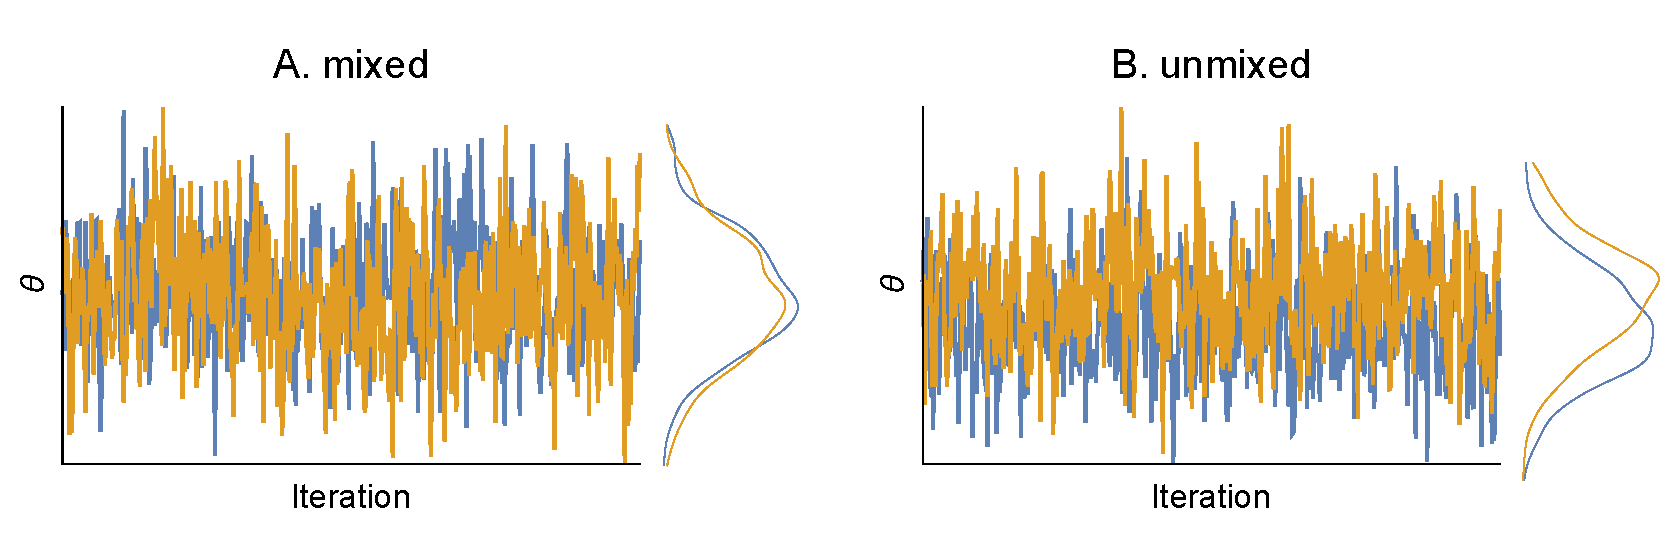
\includegraphics[width=1.0\textwidth]{../output/unmixed_1.pdf}}
	\caption{\textbf{Chain prediction based on the marginal distribution of a single parameter.} A shows the path of two chains that have mixed (to the right of panel); B shows two chains that have not mixed.}
	\label{fig:marginal}
\end{figure}

\begin{figure}[h]
	\centerline{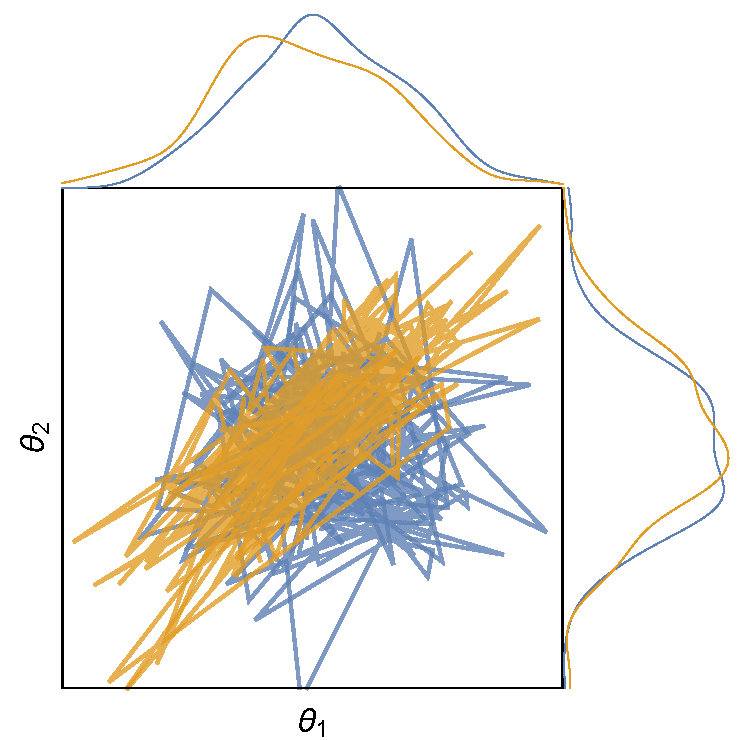
\includegraphics[width=1.0\textwidth]{../output/unmixed_2.pdf}}
	\caption{\textbf{Chain prediction based on the joint distribution of two parameters where each chain's marginals are the same.} A shows the path of two chains that have mixed resulting in similar sampling distributions (to the right and above each panel); B shows two chains that have not mixed.}
	\label{fig:joint}
\end{figure}

These two cases, whilst simple, illustrate the basis of our approach. To determine if a set of Markov chains have converged to the same distribution, we train a supervised machine learning (ML) model to classify the chain to which each sample belongs. By evaluating its performance on an independent test set, we delineate whether chains have mixed based on whether classification accuracy is above the ``null'' case, where accuracy is $1/{N}$, and $N$ is the number of chains. By taking the ratio of ML accuracy to this null accuracy, we obtain a statistic that is interpretable in a similar way to $\hat{R}$ \cite{gelman2013bayesian}. In a nod to this established statistic, we call our statistic $R^*$, and, by design, $R^*\approx 1$ signifies convergence. Algorithm \ref{alg:R_star} gives an explicit recipe for calculating $R^*$.

\begin{algorithm}[tb]
	\caption{$R^*$ calculation}
	\label{alg:R_star}
	\begin{algorithmic}
		\STATE Given chain-wise samples from the target, $\{X^{\{1\}},X^{\{2\}},...,X^{\{N\}}\}$ and a test set length, $S_\text{test}$:
		\FOR{$m=1$ to $N$}
		\STATE Create train and test sets by random-sampling (w/o replacement), $X^{\{m\}}\rightarrow\{X^{\{m\}}_\text{train},X^{\{m\}}_\text{test}\}$
		\ENDFOR
		\STATE Stack $X_\text{train} = (X^{\{1\}}_\text{train},X^{\{2\}}_\text{train},...,X^{\{N\}}_\text{train})^T$
		\STATE Stack $X_\text{test} = (X^{\{1\}}_\text{test},X^{\{2\}}_\text{test},...,X^{\{N\}}_\text{test})^T$
		\STATE Train ML model to classify chain id from any sample, $x$: $\text{ML}(x|X_\text{train}) \rightarrow c$
		\FOR{$s=1$ to $S_\text{test}$}
		\STATE Obtain test sample, $x^{\{s\}}=X_\text{test}(s)\in \mathbb{R}^K$
		\STATE Predict chain id, $c^{\{s\}} = \text{ML}(x^{\{s\}}|X_\text{train})$
		\STATE Compare with actual id, $c^s$: $a^{\{s\}}=\mathbbm{1}(c^{\{s\}}=c^s)$
		\ENDFOR
		\STATE Calculate predictive accuracy, $\bar{a} = \frac{1}{S_\text{test}} \sum_{s=1}^{S_\text{test}} a^{\{s\}}$
		\STATE Calculate ratio to null model accuracy, $R^* = \bar{a} / (1 / N) = N/\bar{a}$
		\RETURN $R^*$
	\end{algorithmic}
\end{algorithm}

The ML model we use here is a gradient-boosted regression tree (also known as a type of gradient-boosted machine or GBM, introduced in \cite{friedman2001greedy}), which experience has dictated to be a highly predictive framework for use in tabular data \cite{chollet2018} like ours. Specifically, we use the GBM implementation in \textbf{\textsf{R}}'s ``Caret'' package \cite{kuhn2008building}, which, in turn, uses the ``gbm'' package \cite{greenwell2019package}. The data for each chain has dimensions: $X\in \mathbb{R}^{S}\times \mathbb{R}^{K}$, where $S$ is the number of samples taken (here assumed the same for each chain, but this is not a binding constraint) and $K$ is the number of parameters. We split each chain's samples into randomly sampled training and testing tests: here, we use 70\% of samples for training and 30\% for testing. The GBM model we use was found to be rapid to execute training then prediction on the testing set (taking $<1$ second on a desktop computer for both these steps for models with 1000 samples), and its predictive performance was insensitive to its hyperparameters. In all the examples explored in \S\ref{sec:results}, the GBM hyperparameter settings we used were: an interaction depth of 3, a shrinkage parameter of 0.1, 10 observations being the minimum required for each node, and that 50 trees would be grown (see \url{https://github.com/ben18785/ml-mcmc-convergence} to replicate this functionality).

A benefit of most ML approaches to classification is that they can output class probabilities, opposed to a single predicted class, which we leverage to produce an uncertainty distribution for $R^*$. Algorithm \ref{alg:R_star_uncertainty} gives a recipe for generating samples from this distribution, which we now elaborate on in words. For each sample, $s$, in our testing set, GBM outputs a simplex of chain probabilities: $\boldsymbol{p}^{\{s\}}=(p_1^{\{s\}},p_2^{\{s\}},...,p_N^{\{s\}})$, which forms a categorical distribution that can be sampled from to yield a unique chain prediction, $c^{\{s\}}$. By comparing this classification to the true classification, $c^s$, we obtain a binary measure, $a^{\{s\}}=\mathbbm{1}(c^{\{s\}}=c^s)$, of whether this prediction was correct. We repeat this process for each sample in the testing set, generating $\boldsymbol{a}=(a^{\{1\}},a^{\{2\}},...,a^{\{N_\text{test}\}})$, whose average yields a single $R^{*\{i\}}=N/\bar{a}$ estimate for iteration $i$. We then iterate this process, for $i=1,2,...,I$, producing a set of $(R^{*\{1\}},R^{*\{2\}},...,R^{*\{I\}})$, which collectively represent a distribution for $R^*$. 


\begin{algorithm}[tb]
	\caption{Procedure to generate $I$ samples of $R^*$}
	\label{alg:R_star_uncertainty}
	\begin{algorithmic}
		\STATE Given test data $X_\text{test}$, number of chains $N$, number of iterations $I$, and fitted
		\STATE model, $\text{ML}(x|X_\text{train})\rightarrow(p_1,p_2,...,p_N)$:
		\FOR{$i=1$ to $I$}
		\FOR{$s=1$ to $S_\text{test}$}
		\STATE Obtain test sample, $x^{\{s\}}=X_\text{test}(s)\in \mathbb{R}^K$
		\STATE Predict chain id probabilities, $(p_1^{\{s\}},p_2^{\{s\}},...,p_N^{\{s\}})= \text{ML}(x^{\{s\}}|X_\text{train})$
		\STATE Draw a chain id, $c^{\{s\}} \sim \text{categorical}(p_1^{\{s\}},p_2^{\{s\}},...,p_N^{\{s\}})$
		\STATE Compare with actual id, $c^s$: $a^{\{s\}}=\mathbbm{1}(c^{\{s\}}=c^s)$
		\ENDFOR
		\STATE Calculate predictive accuracy, $\bar{a} = \frac{1}{S_\text{test}} \sum_{s=1}^{S_\text{test}} a^{\{s\}}$
		\STATE Calculate ratio to null model accuracy, $R^{*i} = \bar{a} / (1 / N) = N/\bar{a}$
		\ENDFOR
		\RETURN $(R^{*1},R^{*2},...,R^{*I})$
	\end{algorithmic}
\end{algorithm}

\section{Results}\label{sec:results}
To illustrate the versatility of $R^*$, we use examples from \cite{vehtari2019rank} with one additional example: the multivariate normal model described in \cite{hoffman2014no}.

\subsection{Heterogeneity in chain variance: autoregressive example}\label{sec:heterogeneity}
We generate four Markov chains, where each samples from an autoregressive order 1 (AR1) process of the form,
%
\begin{equation}
X_t = \rho X_{t-1} + \epsilon_t
\end{equation}
%
where $\epsilon_t\stackrel{i.i.d.}{\sim}\mathcal{N}(0, \sigma)$ and $t=1,2,...,1000$. Three of the chains share the same $\sigma=1$, whereas the other chain has $\sigma=1/3$, so that it has $1/3$ of the (unconditional) variance of the others. In Fig. \ref{fig:ar1}A, we show how a GBM model fitted to these data classifies observations according to a sample's value. Unsurprisingly, since the fourth chain has a smaller variance, observations close to zero are likely to be classified as being generated by this chain.

To illustrate the consistency of $R^*$, we perform 1000 replicates where, in each case, we generate four $\{X_t\}$ series as described (i.e. with one chain with a lower variance). We then fit a gradient-boosted model to a labelled training set of 2800 randomly chosen samples. The fitted model is then used to classify samples in an independent test set (comprising the remaining 1200 observations) according to the chain which generated them. For each replicate, we then calculate $R^*$ as described in Algorithm \ref{alg:R_star}. In Fig. \ref{fig:ar1}B, we show that the accuracy ratio is well above 1 for all replicates.

\begin{figure}[h]
	\centerline{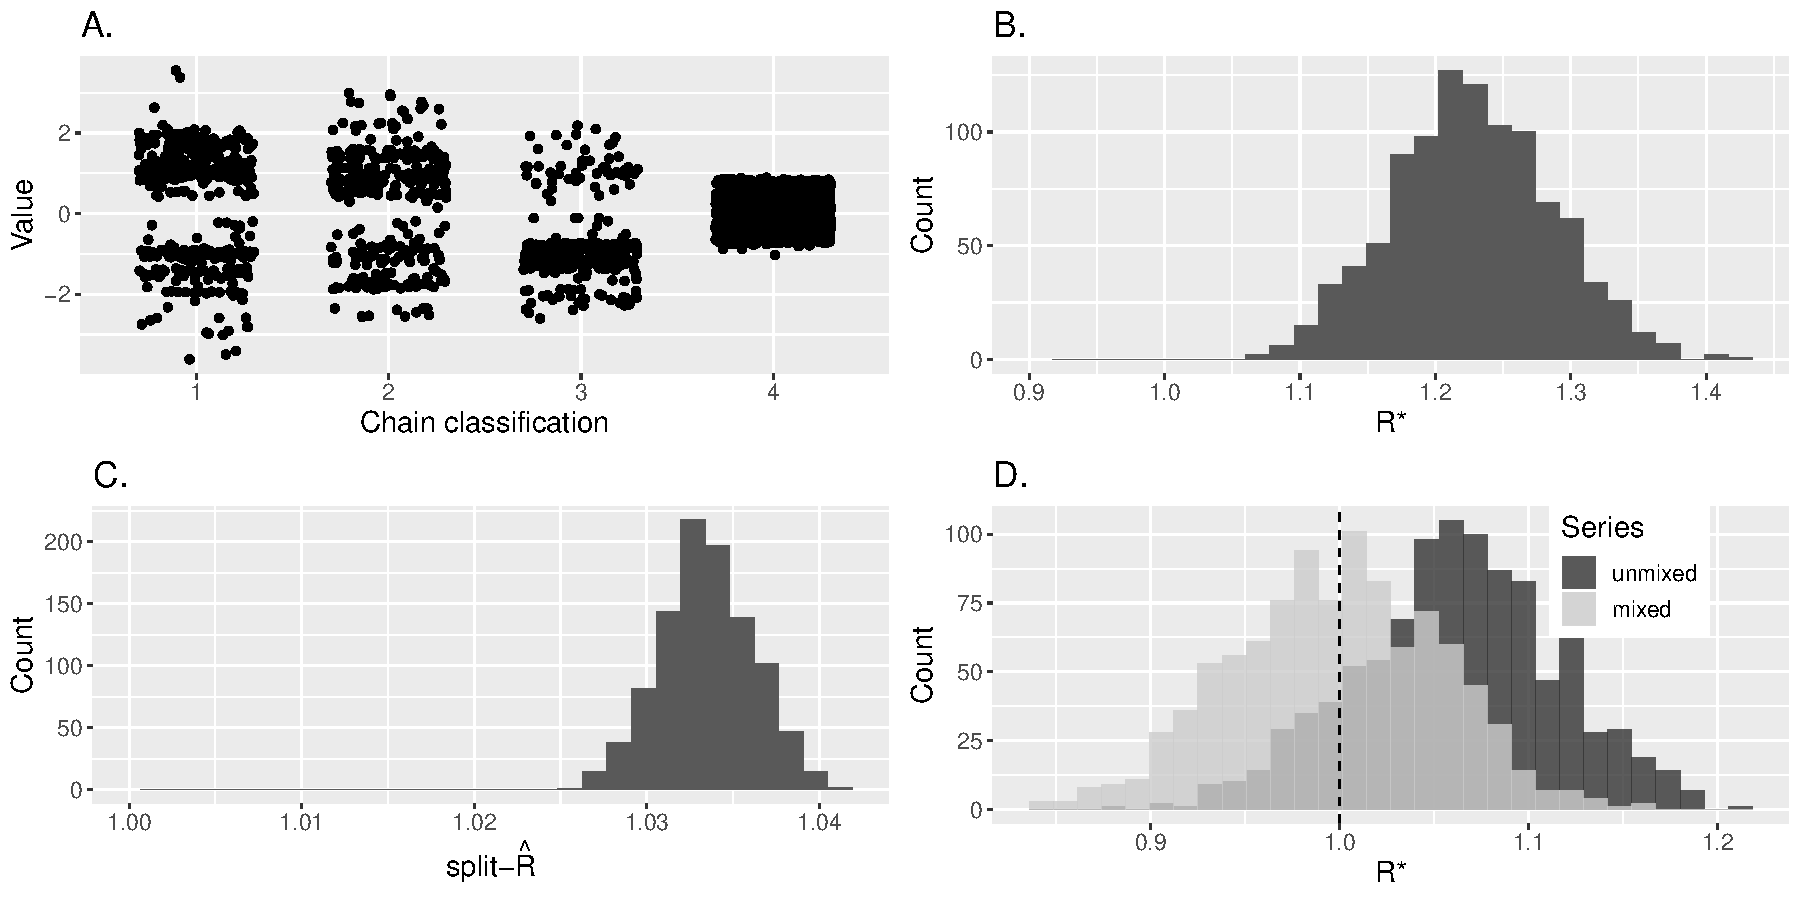
\includegraphics[width=1.0\textwidth]{../output/ar1.pdf}}
	\caption{\textbf{Autoregressive example.} A shows how the GBM's classifications vary according to the sample's value for an example model fit; B shows the calculated $R^*$ values across 1000 replicates; C shows the $R^*$ distributions for the two series described in the text. See the R markdown file on the Github repository for code to reproduce this example.}
	\label{fig:ar1}
\end{figure}

Since GBMs return a probability simplex for each sample, which, for each chain, indicates the probability that a sample was generated by it, we can also generate a measure of uncertainty in $R^*$. Algorithm \ref{alg:R_star_uncertainty} describes in detail how this can be done. We demonstrate this idea using two datasets: one generated as described above, where one chain (out of four) has a lower variance than the others (we call this the ``unconverged'' data'); and another, where all chains sample from the same distribution (we call this the ``converged'' data). In Fig. \ref{fig:ar1}C, we show the $R^*$ distributions in each case. For the unconverged data, the distribution has its bulk of mass away from 1, indicating lack of convergence. For the converged data, the distribution is centred on 1, indicating convergence. 

\subsection{Diagnosing unconvergence in joint distribution: bivariate normal model}\label{sec:bivariate_normal}


\subsection{Slow joint distribution convergence: 250-dimensional multivariate normal model}\label{sec:multivariate_normal}
In this example, we use a 250-dimensional multivariate normal target, where its precision matrix, $\boldsymbol{A}\in\mathbb{R}^{250}\times\mathbb{R}^{250}$, is generated from a Wishart distribution \cite{hoffman2014no}. We assume that the Wishart distribution's degrees of freedom parameter is 250, resulting in a distribution with high correlations between dimensions. We use Stan's NUTS algorithm to sample from this target distribution, and run the algorithm for two different iteration counts (each time across 4 chains): 400 and 10,000 (thinned by a factor of 5). First, we used the ``centered'' parameterisation of this model, which is of the form,
%
\begin{equation}
\boldsymbol{x}\sim \mathcal{N}(\boldsymbol{0},\boldsymbol{A}^{-1}),
\end{equation}
%
where $\boldsymbol{x}\in\mathbb{R}^{250}$. For each set of samples, we used Algorithm \ref{alg:R_star_uncertainty} to generate an uncertainty distribution for $R^*$, which are shown in Fig. \ref{fig:mvt}A. From the plot for the 400 iteration case, it is clear that convergence has not yet occurred since $R^*>1$ across the bulk of this distribution. Even in the 10,000 iteration case, the $R^*$ distribution remains stubbornly shifted a little rightwards of $R^*=1$ (it's mean is 1.02): in this case, $\hat{R}<1.01$ for all parameters, although 61\% of parameters had an $\text{ESS}<400$ indicating issues with convergence \cite{vehtari2019rank}.

Rather than run the MCMC sampler for more iterations, we move to a ``non-centered'' parameterisation, which introduces auxillary variables $\boldsymbol{z}\in\mathbb{R}^{250}$ that don't affect $p(\boldsymbol{x})$ but facilitate sampling from it. This model has the form,
%
\begin{align}
\boldsymbol{A}^{-1} = \boldsymbol{L}\boldsymbol{L}^T,\qquad
\boldsymbol{x} = \boldsymbol{L} \boldsymbol{z},\qquad
z_j\sim \mathcal{N}(0, 1), \text{ for } j = 1,2,...,250.
\end{align}
%
where $\boldsymbol{L}$ is the Cholesky decomposition of the covariance matrix, $\boldsymbol{A}^{-1}$. Fig. \ref{fig:mvt}A shows the $R^*$ distribution resultant from 10,000 NUTS iterations in this case: now the distribution is centred on $R^*=1$ (mean $R^*=1.00$) indicating convergence. This was also reiterated by the fact that $\hat{R}<1.01$ and $\text{ESS}>400$ for all parameters.

In GBMs, it is possible to calculate variable importance (see, for example, \cite{friedman2001greedy} and \cite{greenwell2019package}), and this allows us to determine which variables were mostly responsible for predictive power. We now compare these with the more established metrics $\hat{R}$ and ESS as calculated in Stan. For a GBM fitted to the centered model, we plot in Fig. \ref{fig:mvt}B variable importance (here high values mean a variable is more important) versus $\hat{R}$ for all dimensions of the target distribution (including Stan's $lp$ quantity, shown as a triangle). From this plot, there appears a weak positive association between GBM's variable importance and $\hat{R}$, although the ranked correlation is not significant (Spearman's rank correlation: $\rho=0.05, S=2468800, p=0.35$). In Fig.  \ref{fig:mvt}C, we plot variable importance versus ESS, which exhibit a strong non-linear negative association (Spearman's rank correlation: $\rho=-0.54, S=4060003, p<0.01$). Together, these plots illustrate that the GBM's variable importance measure provides complementary information to $\hat{R}$ and ESS.

\begin{figure}[h]
	\centerline{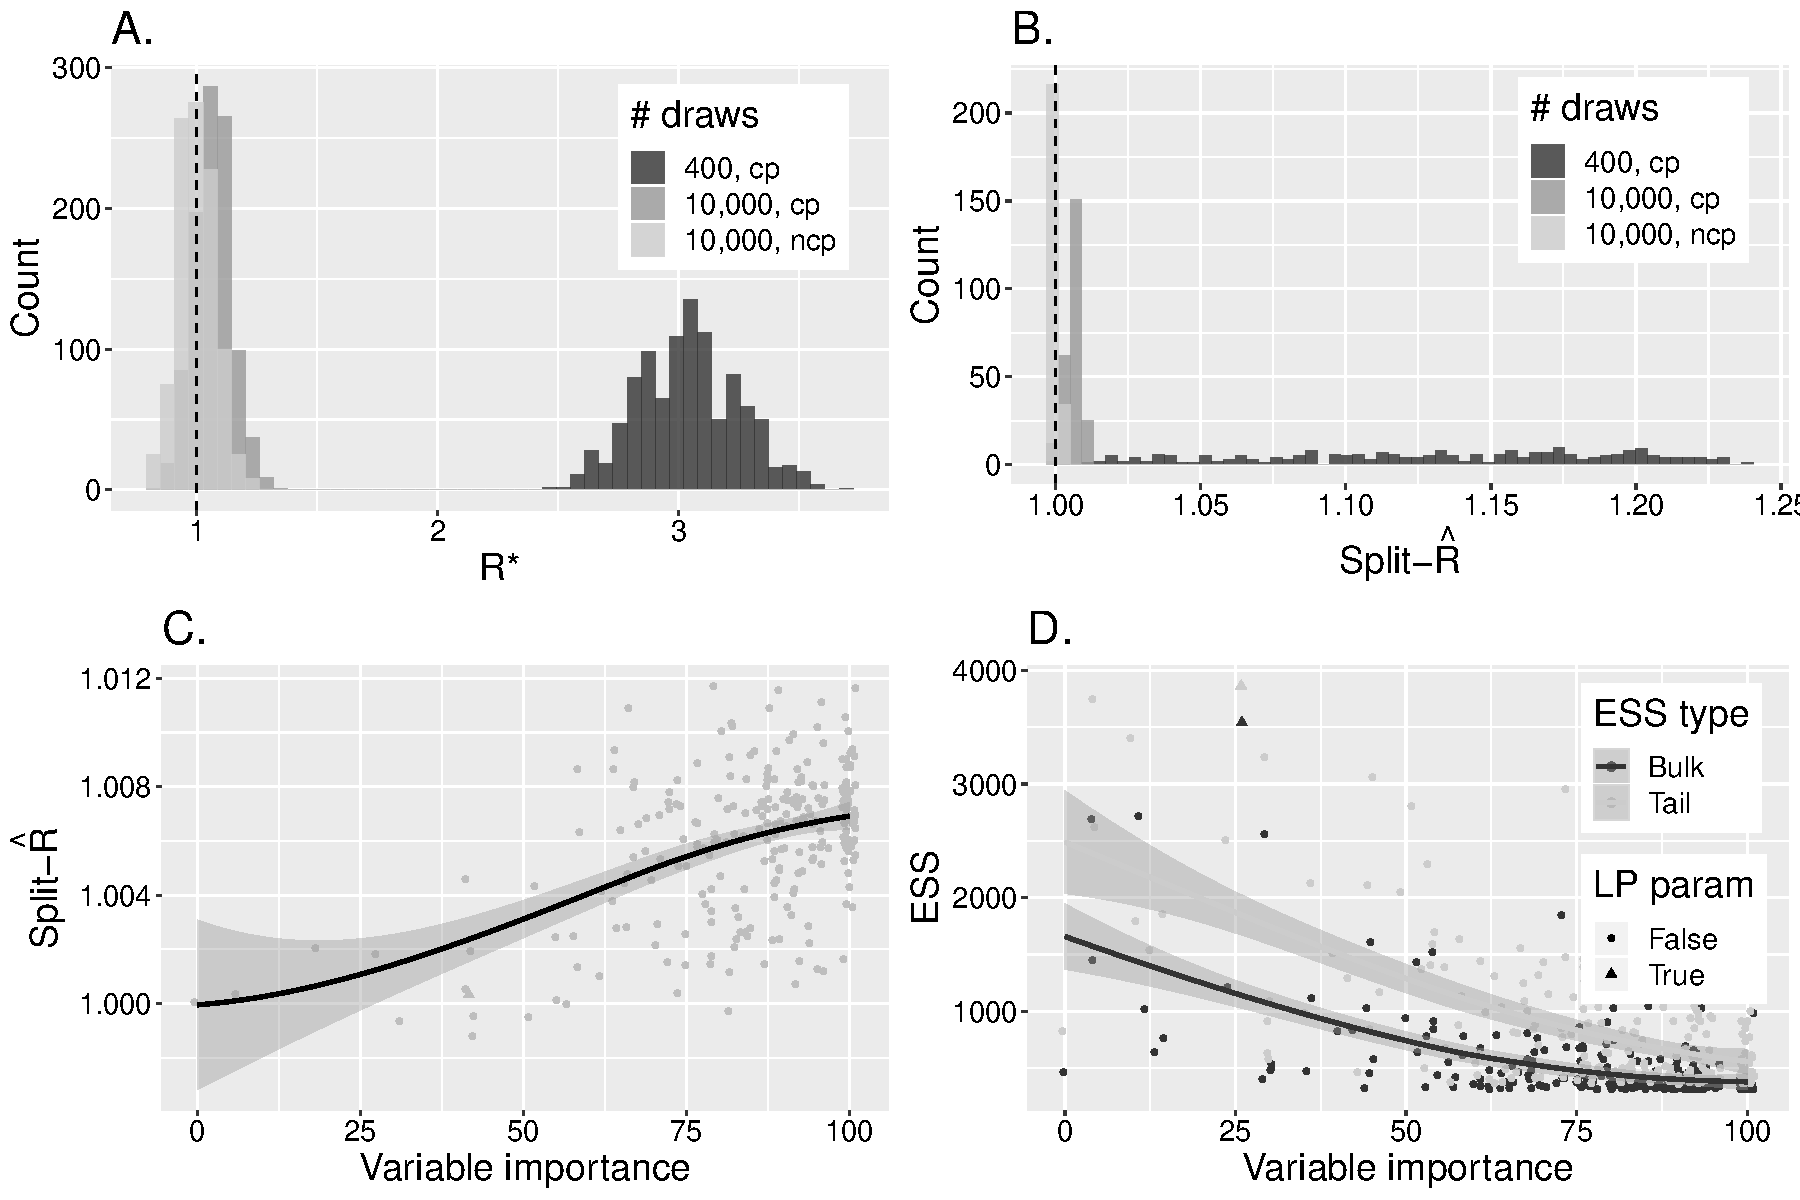
\includegraphics[width=1\textwidth]{../output/mvt_three.pdf}}
	\caption{\textbf{Multivariate normal example.} A shows $R^*$ distributions obtained for two MCMC samples from the centered parameterisation (``cp'') and one from the non-centered version (``ncp''); B shows variable importance versus $\hat{R}$ as calculated by Stan; and C shows variable importance versus ESS as calculated by Stan. In plots B and C, horizontal jitter was added to the points. See the R markdown file on the Github repository for code to reproduce this example.}
	\label{fig:mvt}
\end{figure}

\subsection{Infinite variance: Cauchy example}
We next explore how $R^*$ can be used to determine convergence for distributions with infinite variance. Like \cite{vehtari2019rank}, we first use Stan to sample from independent standard Cauchy distributions for each element of a 50-element vector $x$,
%
\begin{equation}
x_j\sim \text{Cauchy}(0, 1),\; \text{for } j=1,...,50,
\end{equation}
%
We call this parameterisation the ``nominal'' version of this model.

In addition, we also use Stan to sample from an ``alternative'' parameterisation of the Cauchy, based on a scale mixture of Gaussians \cite{vehtari2019rank},
%
\begin{align}
a_j \sim  \N(0,1), \qquad
b_j \sim  \text{Gamma}(0.5, 0.5), \qquad
x_j =  a_j/\sqrt{b_j}.
\end{align}
%
The distribution of the $x$ vector is the same under both parameterisations, although the thin-tailed $(a,b)$ vectors define a higher dimensional posterior that improves sampling efficiency.

In Fig. \ref{fig:cauchy}A, we show the $R^*$ distribution under both parameterisations. As shown in \cite{vehtari2019rank}, the nominal parameterisation results in poor sampling efficiency due to its long tails, meaning that, after 2000 MCMC iterations, samples still contain information about chain identity, and, accordingly, the $R^*$ distribution is shifted rightwards from $R^*=1$. The alternative parameterisation fares better and the $R^*$ distribution is nearer $R^*=1$. Interesting, however, in contrast to the measures presented in \cite{vehtari2019rank}, the $R^*$ distribution for the alternative parameterisation has a mean above 1, indicating that more MCMC iterations are needed: in Fig. \ref{fig:cauchy}B, we show the result for running each Stan model for ten times as long (and thinning by a factor of 5). In this figure, the alternative parameterisation now has an $R^*$ distribution centered on $R^*=1$ and, hence, we are more confident that convergence has been reached. Despite the added iterations, the $R^*$ distribution from the nominal model remains stubbornly away from 1.

\begin{figure}[h]
	\centerline{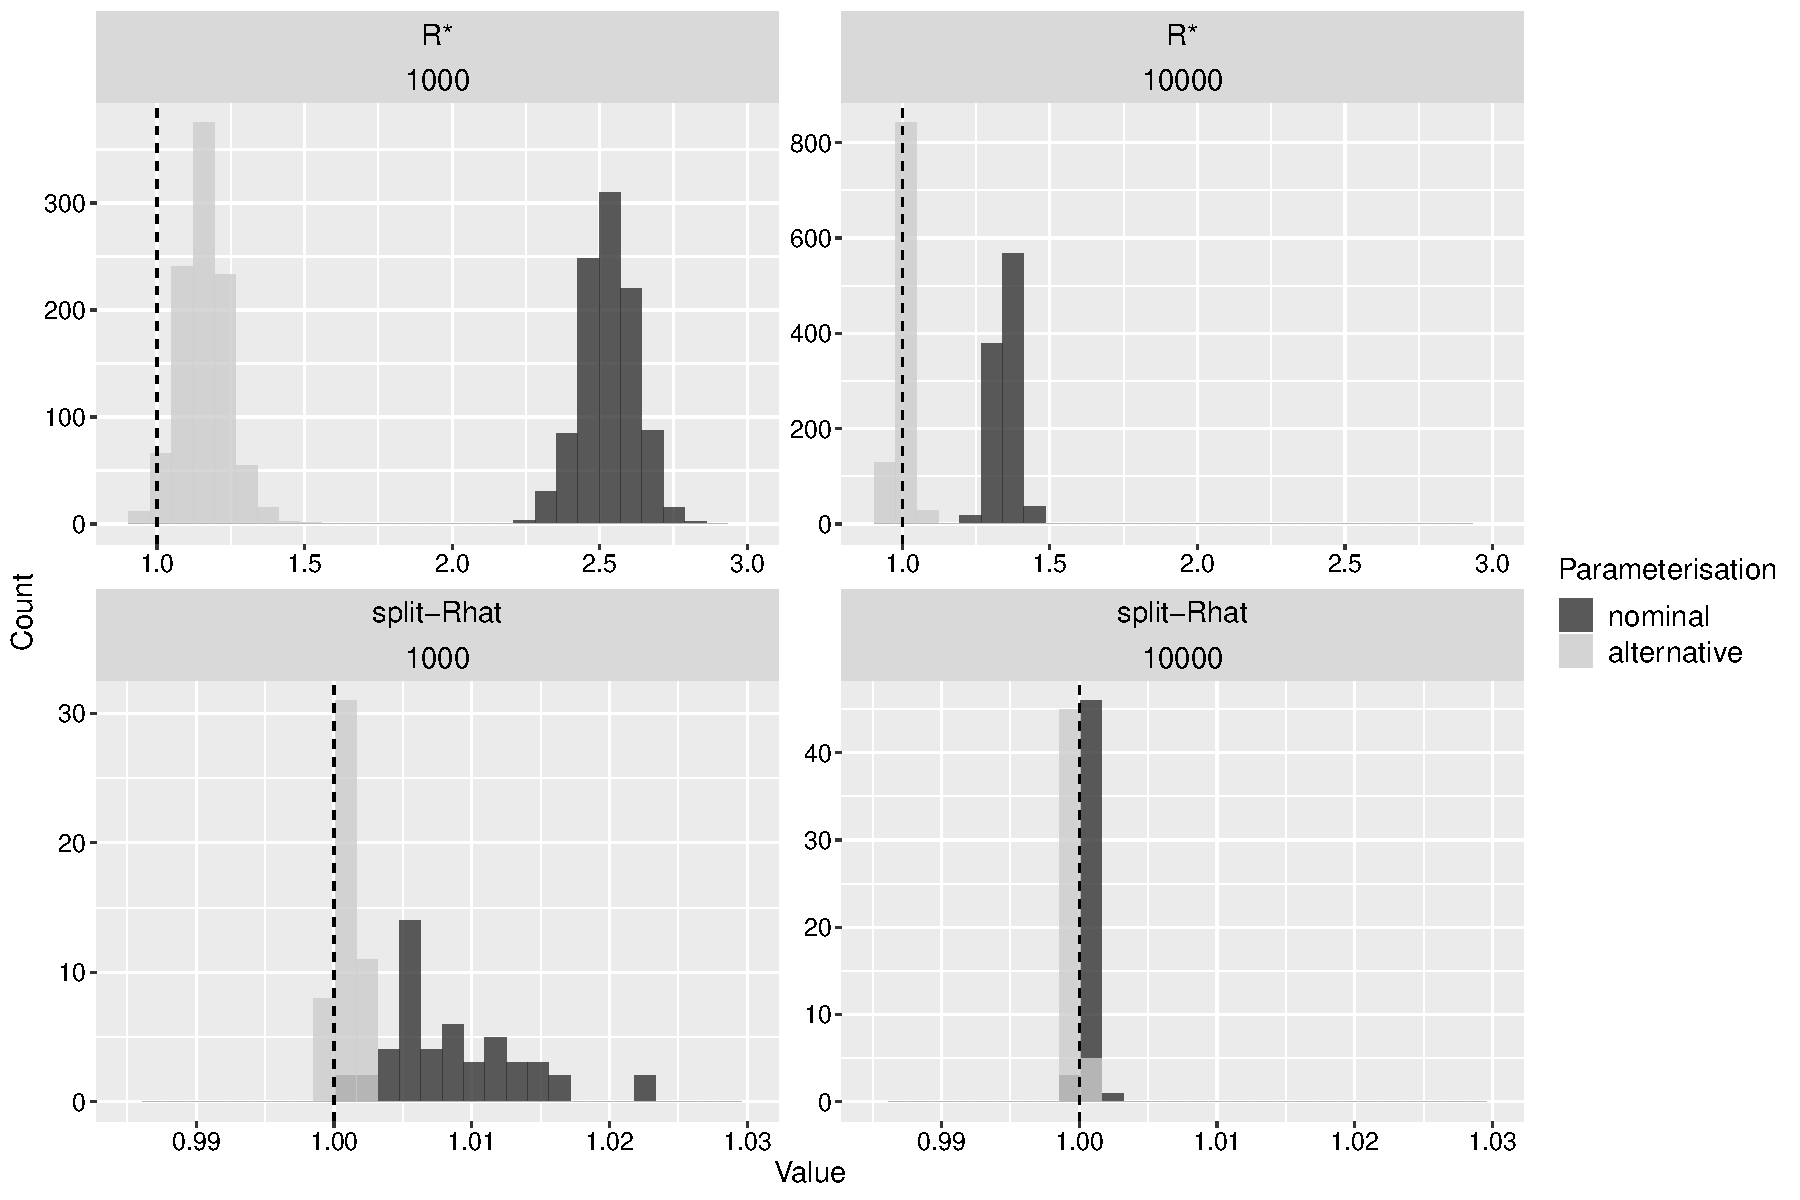
\includegraphics[width=1.0\textwidth]{../output/cauchy.pdf}}
	\caption{\textbf{Cauchy example.} A shows 1000 MCMC samples from the $R^*$ distribution generated under two model parameterisations; B shows the same but with 10,000 MCMC samples used (which are then thinned by a factor of 5). See the R markdown file on the Github repository for code to reproduce this example.}
	\label{fig:cauchy}
\end{figure}

\subsection{Hierarchical model: Eight schools model}\label{sec:eight_shools}
We now examine a simple classic example used to highlight difficulties in performing inference for hierarchical models: referred to as the ``Eight school'' model (see Section 5.5 in \cite{gelman2013bayesian}), which aimed to determine the effects of coaching on SAT scores in eight schools. 

The model can be parameterised two ways, as described in \cite{vehtari2019rank}. The simplest way is referred to as the ``centered'' parameterisation and exactly mirrors the underlying statistical model,
%
\begin{align*}
\theta_j &\sim \N(\mu, \tau) \\
y_j &\sim \N(\theta_j, \sigma_j).
\end{align*}
%
The ``non-centered'' parameterisation recodes this model in a way which does not affect the joint distribution of $(\theta, \mu, \tau, \sigma)$ but makes it easier to sample from it, by introducing auxillary variables, $\tilde \theta_j$. This can be written as,
%
\begin{align*}
\tilde{\theta}_j &\sim \N(0, 1) \\
\theta_j &= \mu + \tau \tilde{\theta}_j \\
y_j &\sim \N(\theta_j, \sigma_j).
\end{align*}
%
In both cases, $\theta_j$ are the treatment effects in the eight schools, and $(\mu, \tau)$ represent the population mean and standard deviation 
of the distribution of these effects. In the centered parameterization, the $\theta_j$ are parameters, whereas in the non-centered parameterization, the $\tilde{\theta}_j$ are parameters and $\theta_j$ is a derived quantity.

We first used Stan \cite{carpenter2017stan} to sample from the centered model using 4 chains. Like \cite{vehtari2019rank}, we use settings that reduce the chance of divergent iterations for the NUTS algorithm \cite{hoffman2014no}, meaning that the resultant sampling distribution is likely to be biased. We also used Stan with the same algorithm settings to sample from the non-centered model.

To see how $R^*$ performed on this example, we first split each of the (post-warm-up) chains in two, as is done by default in Stan \cite{carpenter2017stan} and in \cite{vehtari2019rank}, resulting in 500 iterations across 8 chains. Next, we trained the GBM on a training set comprising 2800 samples, and used it to classify the causative chain for 1200 independent test samples. Following the same approach as in Algorithm \ref{alg:R_star_uncertainty}, we generated $R^*$ distributions for both the centered and non-centered models. The resultant distributions for $R^*$ are shown in Fig.\ref{fig:eight_schools}A. In this plot, it is clear that whereas the centered model shows signs of convergence, the non-centered model does not: intuitively, the chains have not sufficiently mixed with themselves nor the others meaning that the causative chain can be predicted with reasonable accuracy from the sample location.

As in \S\ref{sec:multivariate_normal}, we calculated a measure of variable importance to understand which variables contributed most to the predictive power of the model. For the GBM fitted to the centered model, the most important variable was $\tau$, followed by Stan's $lp$ variable (we also include this in our training and testing data), followed by $\mu$ and $\theta_2$. Interestingly, these were ordered differently according to Stan's $\hat{R}$, with $lp$ having the highest value ($\hat R = 1.06$), followed by $\tau$ ($\hat R = 1.02$), then a host of variables with ($\hat R = 1.01$).

In addition, to illustrate the power of $R^*$, we also repeat the analysis but, this time, do not split the chains in two. The results are shown in Fig.\ref{fig:eight_schools}B. In this case, because the unsplit chains do not mix with themselves, it is harder to accurately predict the chain that generated each sample, meaning that the centered model $R^*$ values are shifted leftwards. Despite this, however, the distribution for $R^*$ still does not strongly overlap with $R^*=1$, indicating that the model has not converged.

\begin{figure}[h]
	\centerline{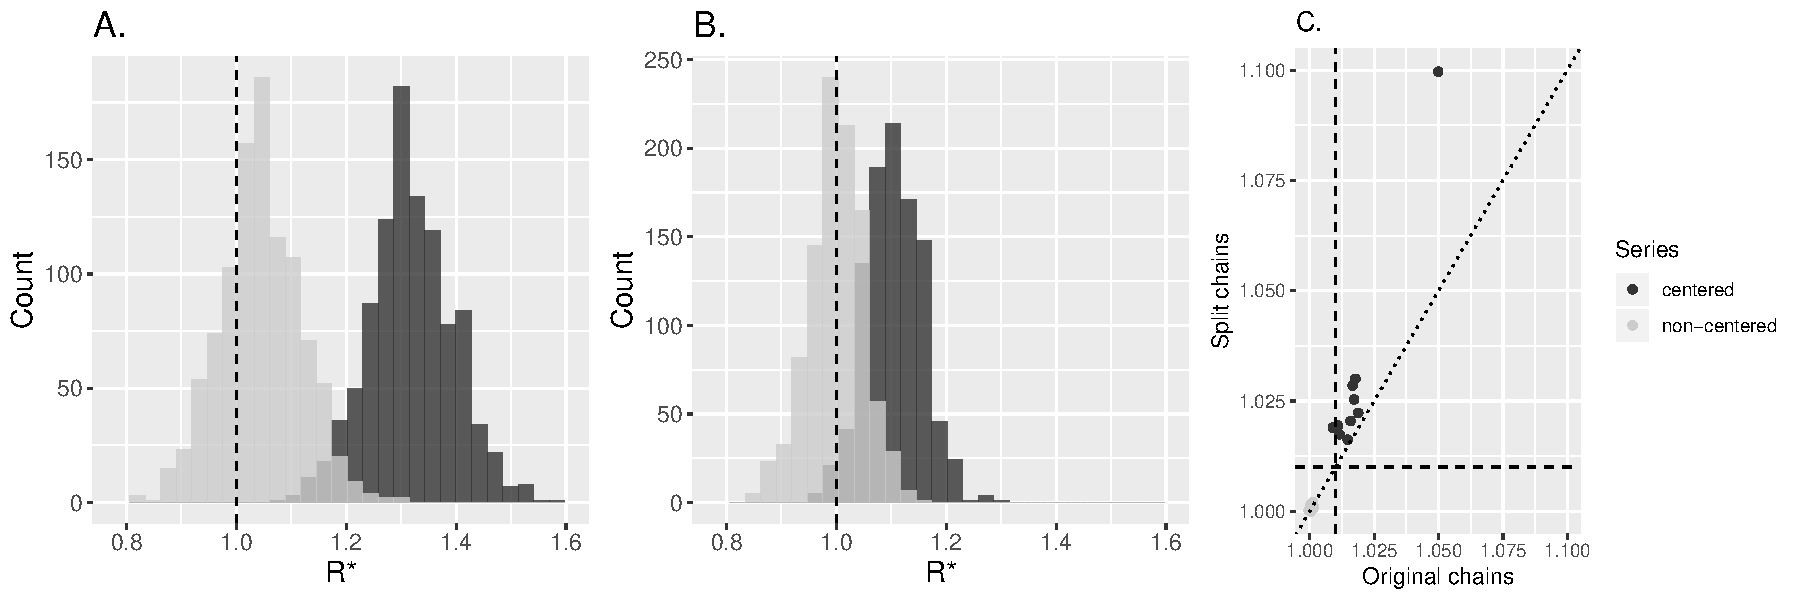
\includegraphics[width=1.0\textwidth]{../output/eight_schools.pdf}}
	\caption{\textbf{Eight schools example.} A shows samples from the $R^*$ distribution when splitting chains in two (resulting in 8 chains); B shows the same but using the 4 original chains. In both cases, the plots show 1000 $R^*$ samples. See the R markdown file on the Github repository for code to reproduce this example.}
	\label{fig:eight_schools}
\end{figure}

\section{Discussion}
If an MCMC sampler has converged on the target distribution, the chains must be well ``mixed'', that is, given a sample it should be impossible to discern which chain generated it. Based on this observation, we used supervised machine learning (ML) models to quantify the information about the generative chain identity contained in samples. By taking the ratio of ML model predictive accuracy obtained on an independent test set to the accuracy of a null model (which predicts a chain's identity uniformly at random), this defines our $R^*$ statistic. By extracting ML-predicted chain probabilities from each prediction in the test set, we can additionally generate an uncertainty distribution for $R^*$. Across a range of previously published examples, $R^*$ was shown to be predictive of whether or not chains had converged.

The predominant methods for diagnosing MCMC convergence rely heavily on looking for between-chain differences in the marginal distributions along each dimension. $R^*$ naturally includes this information in building a model capable of predicting the chain which generated each sample. It also naturally includes information about the joint distribution across all dimensions of the target. Since converged chains should have similar joint distributions (implying similar marginals), any measure of convergence should account for both of these aspects. Indeed, in \S\ref{sec:multivariate_normal}, we show that more established measures may indicate converge whereas $R^*$ shows otherwise. This is not a sleight on existing measures, more that we argue this illustrates the complementarity of $R^*$ to them.

When first starting to develop $R^*$, it was unclear to us whether \textit{any} metric aligned with a supervised ML method would be overly sensitive to its hyperparameters. With gradient-boosted regression tree models, we found this not to be the case. Indeed, after a little experimenting, we found that a single set of hyperparameters (which we report in \S\ref{sec:method}) sufficed across all our examples. To ensure maximal predictive capability of any fitted ML model, however, it is prudent to optimise it over choice of hyperparameters, and we recommend that applied users consider including this step in their workflow.

Many implementations of $\hat{R}$ suggest splitting chains in two before calculating it. In the Eight Schools example in \S\ref{sec:eight_shools}, we trial this before calculating $R^*$, and find that this approach leads to more accurate chain prediction. As such, we recommend that this practice be adopted whenever $R^*$ is calculated to ensure that this measure is maximised. Additionally, our ML calculation method for $R^*$ makes it possible to include any covariates which may be useful features for prediction, such as an ``iteration block'' indicator variable taking values $1, 2, ..., K$ in each of $K$ blocks of contiguous iterations. If each chain is thoroughly mixed with itself, including this additional information shouldn't change $R^*$; by contrast, if the chains are random walk-like, this information should boost $R^*$.

MCMC enables inference across a large range of models encountered across the social, biological and physical sciences. Its ease of implementation, however, masks important underlying fragilities in the method. Namely, that unless the chains have converged to a truly stationary distribution, the samples generated are not faithful depictions of the posterior. In this paper, we introduce a new metric, $R^*$, that is especially good at diagnosing poor convergence in the joint sampling distribution -- an area that we argue has received insufficient attention thus far. $R^*$ can straightforwardly be introduced into existing MCMC libraries and could provide a measure of convergence complementary to existing metrics.

	
\bibliographystyle{unsrt}
\bibliography{bibliography} 
	
\end{document}
